% ==========================================
% BAB IV PERANCANGAN
% ==========================================
\cleardoublepage
\chapter{PERANCANGAN MODEL PENDETEKSIAN TUMOR OTAK BERBASIS CNN YANG TERINTEGRASI XAI}
\label{chap:perancangan}

Secara umum, alur implementasi pada penelitian ini terbagi menjadi empat tahap utama. Pertama, \textit{data understanding} yang mencakup pengumpulan data dari tiga sumber, yaitu citra otak tanpa tumor (\textit{No Tumor Scrape}), citra otak dengan tumor (\textit{Tumor Scrape}), dan citra otak dengan \textit{mask} tumor (\textit{Tumor with Mask}), yang kemudian dibagi menjadi subset \textit{train}, \textit{validation}, dan \textit{test}. Kedua, \textit{data preparation} yang meliputi konversi format, standardisasi saluran RGB, pemilihan \textit{preprocessing} eksperimen (Gaussian+CLAHE atau Wavelet+Normalisasi Intensitas atau tanpa kedua preprocessing tersebut), seleksi \textit{Region of Interest} (ROI), dan augmentasi data. Ketiga, \textit{modelling} yang menguji tiga arsitektur model, yaitu CLM (CNN + ANN), \textit{Explainable} CNN (CNN + Grad-CAM \textit{Pruning}), dan EfficientNetB0, masing-masing dengan \textit{hyperparameter tuning}. Keempat, evaluasi yang mencakup pemilihan model terbaik per arsitektur, dilanjutkan dengan implementasi XAI menggunakan Grad-CAM yang disertai evaluasi XAI menggunakan metrik XAlign.

\begin{figure}[h]
	\centering
	\captionsetup{justification=centering}
	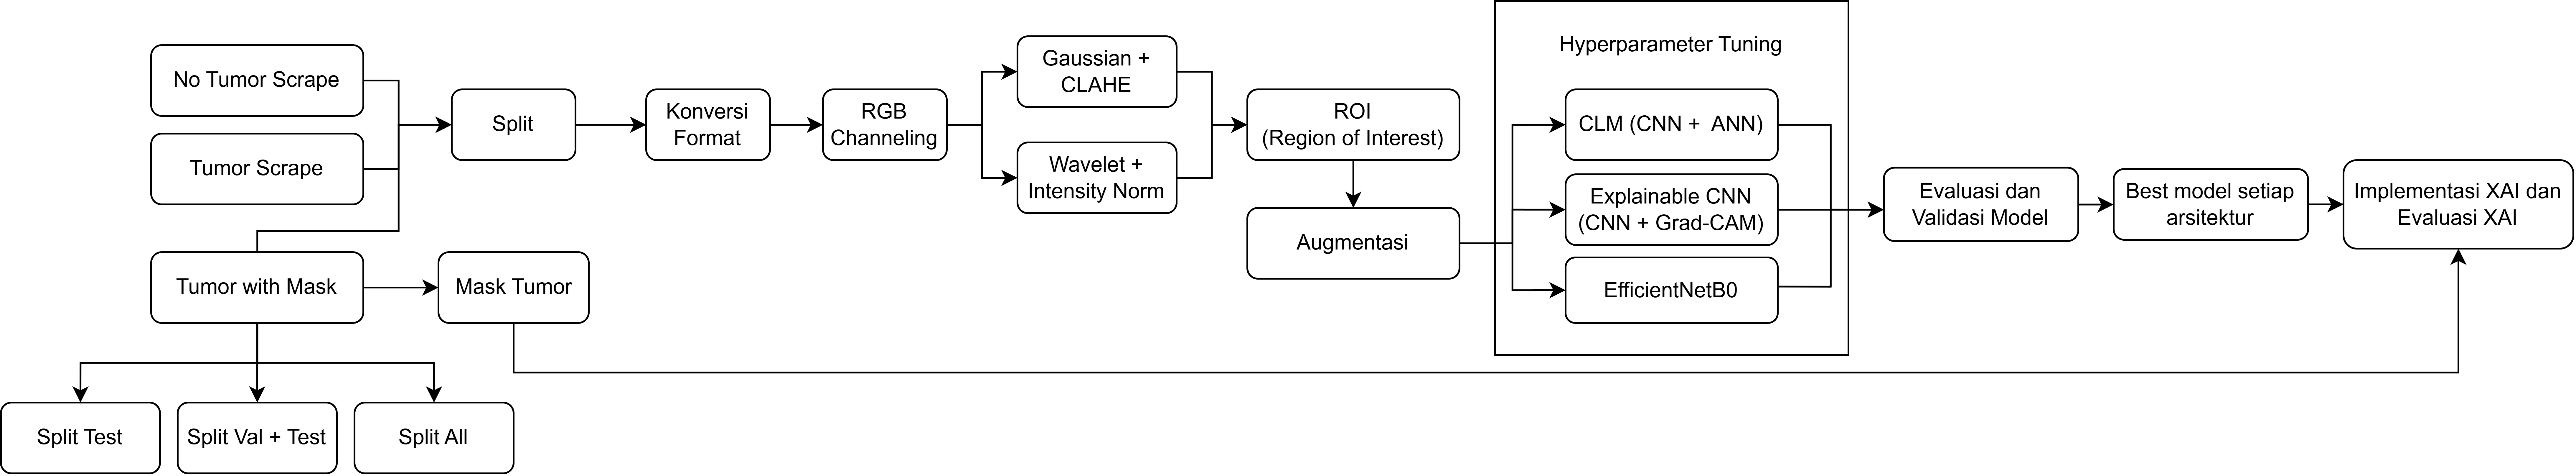
\includegraphics[width=1.0\textwidth]{images/Flow Arsitektur.png}
	\caption{Perancangan Alur Implementasi}
	\label{gambar:arsitekturperancangan}
\end{figure}

\section{\textit{Data Understanding}}
Selain modifikasi arsitektur, penyesuaian juga dilakukan pada \textit{dataset} yang digunakan. \textit{Dataset} yang digunakan dalam tugas akhir ini merupakan gabungan dari dua sumber data yang berbeda untuk menciptakan kumpulan data yang dapat digunakan untuk klasifikasi tumor otak serta segmentasi tumor otak.

\begin{enumerate}
	\item \textit{Dataset} Otak CT \textit{Scan} tanpa \textit{Mask} Tumor
	
	Untuk melatih dan memvalidasi model, Tugas Akhir ini mengumpulkan datast melalui website Radiopaedia. Radiopaedia merupakan repositori kasus pencitraan medis yang mencakup berbagai modalitas, seperti CT-scan dan MRI. Meskipun terbuka dari komunitas medis, seluruh draf artikel dan kasus klinis yang diunggah dapat dilakukan \textit{peer-review} dan harus melewati proses divalidasi oleh para ahli radiologi profesional yang bekerja sama dengan Radiopaedia. Proses verifikasi ini memastikan bahwa setiap data gambar yang tersedia memiliki diagnosis patologi yang akurat dan anotasi klinis yang dapat dipertanggungjawabkan.
	
	\begin{figure}[h]
		\centering
		\captionsetup{justification=centering}
		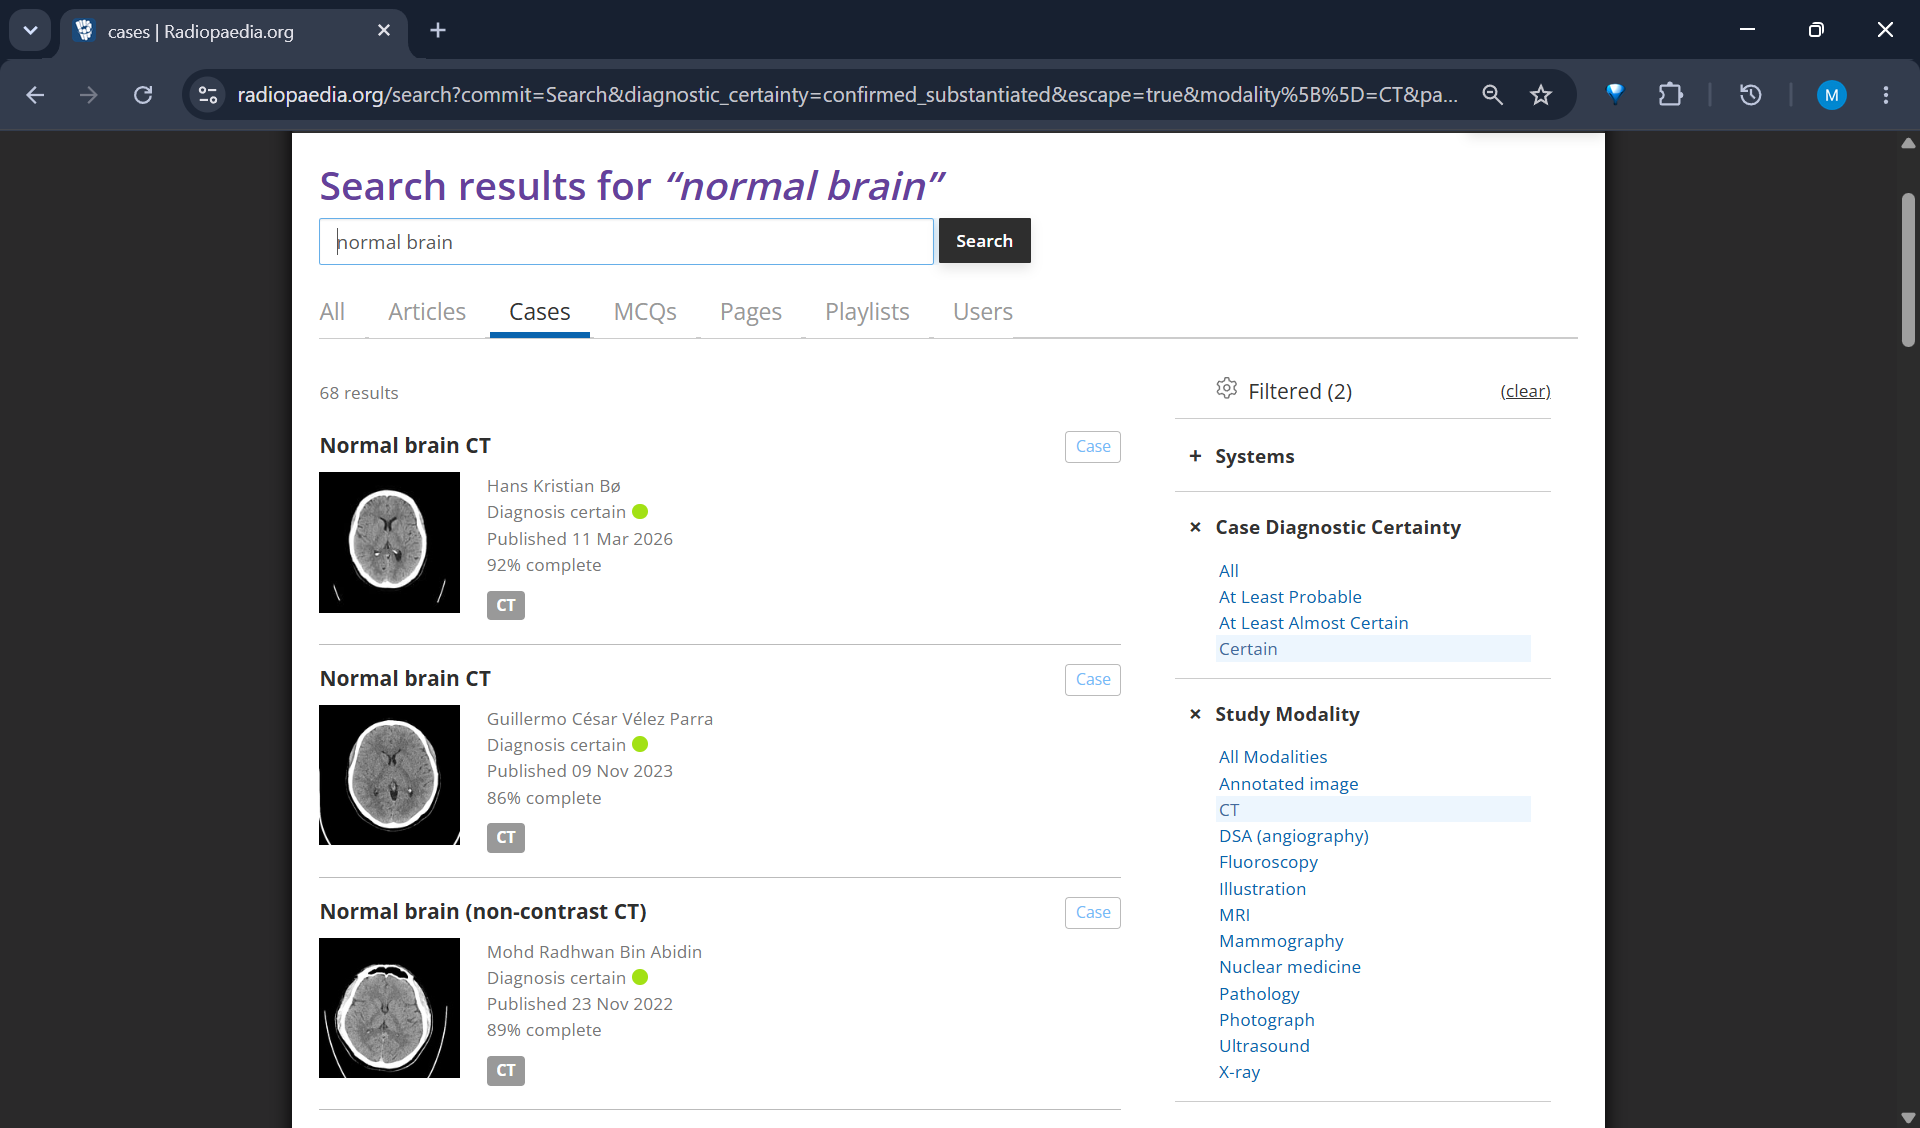
\includegraphics[width=0.85\textwidth]{images/normal brain radio.png}
		\caption{Website Radiopaedia}
		\label{gambar:websiteradiopaedia}
	\end{figure}
	
	Dalam pengumpulan data, dilakukan pencarian secara manual dengan beberapa kata kunci yang dibagi menjadi dua, yaitu normal dan kelas penyakit (glioma dan meningioma). Pada pencarian tersebut, terdapat \textit{filter} modalitas pencitraan berupa CT \textit{scan}) dan dengan bidang \textit{Axial} \textit{non-contrast}. Setelah dilakukan pencarian, dilakukan pengunduhan secara manual dengan melihat letak tumor dari gambar lain, seperti MRI atau anotasi pada gambar yang lain. Dalam pengunduhan, dilakukan pemisahan folder untuk tempat setiap kelas yang akan dijadikan bahan untuk pelatihan dan tes model.
	
	\item \textit{Dataset} Otak CT \textit{Scan} dengan Tumor dan \textit{Mask} Tumor
	
	Untuk \textit{Dataset} Otak dengan Tumor dan \textit{Mask} Tumor, tugas akhir ini menggunakan \textit{dataset} \textit{Unpaired MR-CT Brain Dataset for Unsupervised Image Translation} \cite{AlKadi2022Unpaired}. \textit{Dataset} ini digunakan sebagai \textit{ground truth} untuk kebutuhan validasi XAI. Spesifikasi dari \textit{dataset} yang digunakan adalah:
	
	\begin{enumerate}
		\item Sumber: Jordan University Hospital (via Mendeley Data).
		\item Kondisi Medis: Patologis (tumor otak).
		\item Format Data: Citra 2D (DICOM).
		\item Resolusi Citra: 256 $\times$ 256 piksel.
		\item Representasi Piksel: 8-\textit{bit} (0-255) yang telah diterapkan filter \textit{smooth} dan \textit{sharp}.
		\item Ketebalan \textit{Slice}: 7,0 mm.
		\item Jumlah Sampel: 89 citra CT bidang aksial.
	\end{enumerate}

\end{enumerate}

\section{\textit{Data} \textit{Preparation}}
Dalam melakukan preprarasi pada semua dataset, terdapat \textit{preprocessing} yang dilakukan agar data menjadi seragam dan \textit{preprocessing} tambahan yang dilakukan untuk eksperimen agar model bisa mendeteksi tumor lebih baik. 

\subsection{\textit{Preprocessing} Umum}
Pada penelitian ini, tahap \textit{preprocessing} umum diterapkan pada seluruh citra masukan untuk memastikan kompatibilitas format dasar dengan arsitektur model yang akan digunakan.
\begin{enumerate}
	\item Standardisasi Format dan Saluran:
	Citra masukan yang didapatkan dari berbagai sumber memiliki format yang bervariasi (misalnya \textit{grayscale} atau RGB). Seluruh citra diseragamkan menjadi format \textit{Red-Green-Blue} (RGB) dengan 3 saluran (\textit{channels}). Penyesuaian ini diwajibkan karena sebagian besar arsitektur CNN menerima dimensi masukan awal dengan 3 saluran warna.
	
	\item Penyesuaian Dimensi dan \textit{Padding}:
	Seluruh citra diubah dimensinya menjadi ukuran yang seragam (sebagai contoh $224 \times 224$ atau $256 \times 256$ piksel). Untuk mencegah distorsi rasio aspek anatomis jaringan otak akibat pemampatan (\textit{squishing}), teknik \textit{padding} digunakan. Piksel bernilai nol (hitam) ditambahkan pada sisi citra yang lebih pendek sehingga citra menjadi berbentuk persegi secara proporsional sebelum dilakukan penyesuaian ukuran. Hasil akhir disimpan sebagai file PNG dalam format \textit{unsigned integer} 8-bit (uint8) dengan rentang nilai piksel $[0, 255]$.
	
	\item Seleksi \textit{Region of Interest} (ROI):
	Citra MRI umumnya mengandung latar belakang gelap yang tidak berkontribusi pada proses klasifikasi. Mengacu pada metodologi Islam et al. \cite{islam2024deep}, seleksi ROI dilakukan melalui dua tahap. Pertama, citra dikonversi ke \textit{grayscale} menggunakan persamaan:
	\begin{equation}
		I_g = 0{,}299 \cdot I_R + 0{,}587 \cdot I_G + 0{,}114 \cdot I_B
	\end{equation}
	Kedua, \textit{thresholding} Otsu diterapkan pada citra \textit{grayscale} untuk memisahkan \textit{foreground} dari \textit{background} secara otomatis dengan meminimalkan varian intra-kelas. \textit{Bounding box} terkecil yang mencakup seluruh kontur \textit{foreground} yang valid kemudian dihitung, dan area tersebut di-\textit{crop} dari citra RGB asli sebagai ROI. Pada kasus di mana tidak ditemukan kontur yang valid (ukuran crop $< 32 \times 32$ piksel), citra penuh digunakan sebagai \textit{fallback}.
\end{enumerate}

\subsection{\textit{Preprocessing} Eksperimen}
Preprocessing tambahan dilakukan sesuai dengan beberapa artikel yang tersedia, yaitu sebagai berikut.

\begin{enumerate}
	\item clahe + Gaussian \textit{denoise} (\textcite{putra2025enhanced})
	
	Pemfilteran Gaussian (Gaussian \textit{filtering}) diterapkan pada tahap \textit{denoising} dengan tujuan utama untuk menekan derau frekuensi tinggi (\textit{high-frequency noise}) pada citra MRI. Penerapan filter ini secara langsung dapat meningkatkan rasio sinyal terhadap derau (\textit{signal-to-noise ratio}) pada tekstur gambar. Melalui pengurangan derau ini, representasi visual dari margin (tepi) tumor menjadi lebih jelas dan tingkat kecerahan di seluruh irisan gambar menjadi lebih seragam, sehingga model \textit{Convolutional Neural Network} (CNN) mampu mengekstraksi fitur-fitur tekstur dengan jauh lebih efektif.
	
	Contrast Limited Adaptive Histogram Equalization (CLAHE) diterapkan pada tahap prapemrosesan (\textit{preprocessing}) untuk meningkatkan kontras lokal pada citra. Teknik algoritma ini berfungsi untuk menonjolkan batas-batas tumor secara efektif tanpa ikut mengamplifikasi derau (\textit{noise}) di sekitarnya. Dengan mengoptimalkan kontras secara lokal, penggunaan CLAHE yang digabungkan dengan normalisasi dan reduksi derau memungkinkan jaringan model \textit{deep learning} untuk menangkap fitur-fitur tekstur tumor yang sangat halus (\textit{fine-grained}) dengan lebih akurat.
		
	\item \textit{Wavelet Filter} + \textit{Intensity Normalization} (\textcite{flower2025performance})
	Filter Wavelet merupakan teknik reduksi derau yang mendekomposisi gambar ke dalam beberapa pita frekuensi (koefisien aproksimasi dan detail) melalui transformasi wavelet, sehingga memungkinkan analisis lokal pada komponen waktu maupun frekuensi secara bersamaan untuk menangkap fitur transien dan mengurangi derau. Pada implementasi yang digunakan, dekomposisi dilakukan dengan wavelet Daubechies (\textit{db1}, setara wavelet Haar) level 1, lalu derau ditekan melalui \textit{soft-thresholding} (ambang 0.05) hanya pada koefisien detail, sementara koefisien aproksimasi yang merepresentasikan struktur utama gambar dipertahankan sebelum direkonstruksi kembali per kanal warna (R, G, B) secara independen. Pendekatan ini menjadikan filter wavelet unggul mempertahankan tepi (\textit{edges}) dan struktur anatomi penting sekaligus efektif menghilangkan derau yang tidak diinginkan.
	
	\textit{Intensity Normalization} merupakan teknik \textit{enhancement} yang menstandarkan rentang intensitas piksel pada seluruh dataset, mengurangi variabilitas akibat perbedaan pengaturan mesin pemindai atau protokol akuisisi, sehingga penting untuk menjaga konsistensi antar gambar pada tahap analisis MRI selanjutnya seperti segmentasi maupun klasifikasi. Pada implementasi yang digunakan, normalisasi dilakukan melalui pendekatan \textit{z-score} per kanal warna — mengurangkan nilai piksel dengan \textit{mean} lalu membaginya dengan \textit{std} tiap kanal — yang dihitung khusus dari data \textit{train} (bukan seluruh dataset) untuk mencegah \textit{data leakage} ke subset validasi dan uji. Dengan menstandarkan distribusi intensitas secara konsisten, teknik ini meningkatkan \textit{reliability} dan \textit{reproducibility} hasil pencitraan untuk mendukung tahap deteksi tumor otak selanjutnya.
\end{enumerate}

\subsection{Augmentasi}
Berdasarkan \autocite{goceri2023medical}, menggabungkan beberapa proses augmentasi secara berurutan terbukti memberikan performa klasifikasi yang lebih tinggi dibandingkan dengan augmentasi tunggal. Pada penelitian ini, diterapkan tiga metode augmentasi geometris yang dijalankan hanya pada data \textit{training}, dengan setiap gambar asli menghasilkan 3 salinan augmentasi (1 salinan per metode), sehingga total dataset \textit{training} menjadi 4 kali lipat data asli (1 citra asli ditambah 3 citra hasil augmentasi). Seluruh piksel yang keluar \textit{frame} akibat transformasi diisi menggunakan refleksi tepi (\texttt{BORDER\_REFLECT\_101}) agar tidak terdapat artefak hitam yang dapat mengganggu fitur medis. 

\begin{enumerate} 
	\item \textit{Shearing} Tunggal
	Pada metode ini, citra mengalami distorsi sudut pada sumbu $x$ dan $y$ secara independen dengan sudut yang dipilih secara acak dari rentang $-15^\circ$ hingga $15^\circ$. Pusat transformasi ditetapkan di tengah citra agar lesi tidak bergeser jauh dari posisi aslinya. Pada klasifikasi citra \textit{CT scan} paru, metode ini merupakan augmentasi tunggal yang paling tidak efisien apabila diaplikasikan secara tersendiri tanpa dikombinasikan dengan transformasi lain \autocite{goceri2023medical}.
	
	\item Rotasi Tunggal
	Citra dirotasi searah atau berlawanan arah jarum jam dengan sudut acak dari rentang $-25^\circ$ hingga $25^\circ$, berpusat di tengah citra. Rotasi umumnya aman diterapkan pada citra medis karena lesi dapat muncul pada berbagai orientasi, sehingga model jaringan dapat belajar mengenali fitur yang tidak bergantung pada orientasi tertentu \autocite{goceri2023medical}.
	
	\item Translasi $\to$ \textit{Shearing} $\to$ Rotasi
	Metode ini merupakan kombinasi tiga transformasi geometris yang diterapkan secara berurutan (translasi, \textit{shearing}, kemudian rotasi), menjadikannya metode augmentasi paling komprehensif dalam penelitian ini. Dalam kode implementasi, \textit{pipeline} ini diberi label sebagai metode augmentasi terkuat:
	\begin{enumerate}
		\item Translasi: Citra digeser secara acak dalam rentang $-15$ hingga $15$ piksel pada kedua sumbu untuk mensimulasikan variasi posisi.
		
		\item \textit{Shearing}: Citra yang telah digeser kemudian didistorsi dengan sudut acak antara $-15^\circ$ hingga $15^\circ$ untuk mensimulasikan variasi proyeksional.
		
		\item Rotasi: Terakhir, citra dirotasi dengan sudut acak dari rentang $-25^\circ$ hingga $25^\circ$ untuk mensimulasikan variasi orientasi akuisisi pemindaian.
	\end{enumerate}
	
	Kombinasi ketiga transformasi ini terbukti menjadi pendekatan paling tepat untuk augmentasi citra \textit{MR} otak dalam meningkatkan klasifikasi kasus HGG dan LGG, dengan akurasi sebesar 88.24\%, sensitivitas 90.48\%, dan spesifisitas 97.13\% \autocite{goceri2023medical}.
\end{enumerate}


\section{\textit{Modelling}}

\subsection{Arsitektur Model Correlation Learning Mechanism (CLM)}

Gambar pertama menunjukkan arsitektur umum dari \textit{Correlation Learning Mechanism} (CLM), yang menggambarkan keterkaitan antara CNN dan ANN dalam satu siklus pembelajaran. Pada diagram tersebut terlihat bahwa citra input diproses melalui tahap segmentasi sebelum masuk ke CNN, kemudian hasil filter dari CNN dievaluasi melalui \textit{Evaluation Vector} dan ANN. Hasil evaluasi berupa nilai akurasi, \textit{loss}, dan \textit{shuffle value} disimpan ke dalam \textit{Palettes Archives}, lalu dipilih dan dibangkitkan kembali menjadi konfigurasi palette baru yang dikirim ulang ke CNN, sehingga membentuk mekanisme umpan balik yang berulang selama proses pelatihan berlangsung.

\begin{figure}[h]
	\centering
	\captionsetup{justification=centering}
	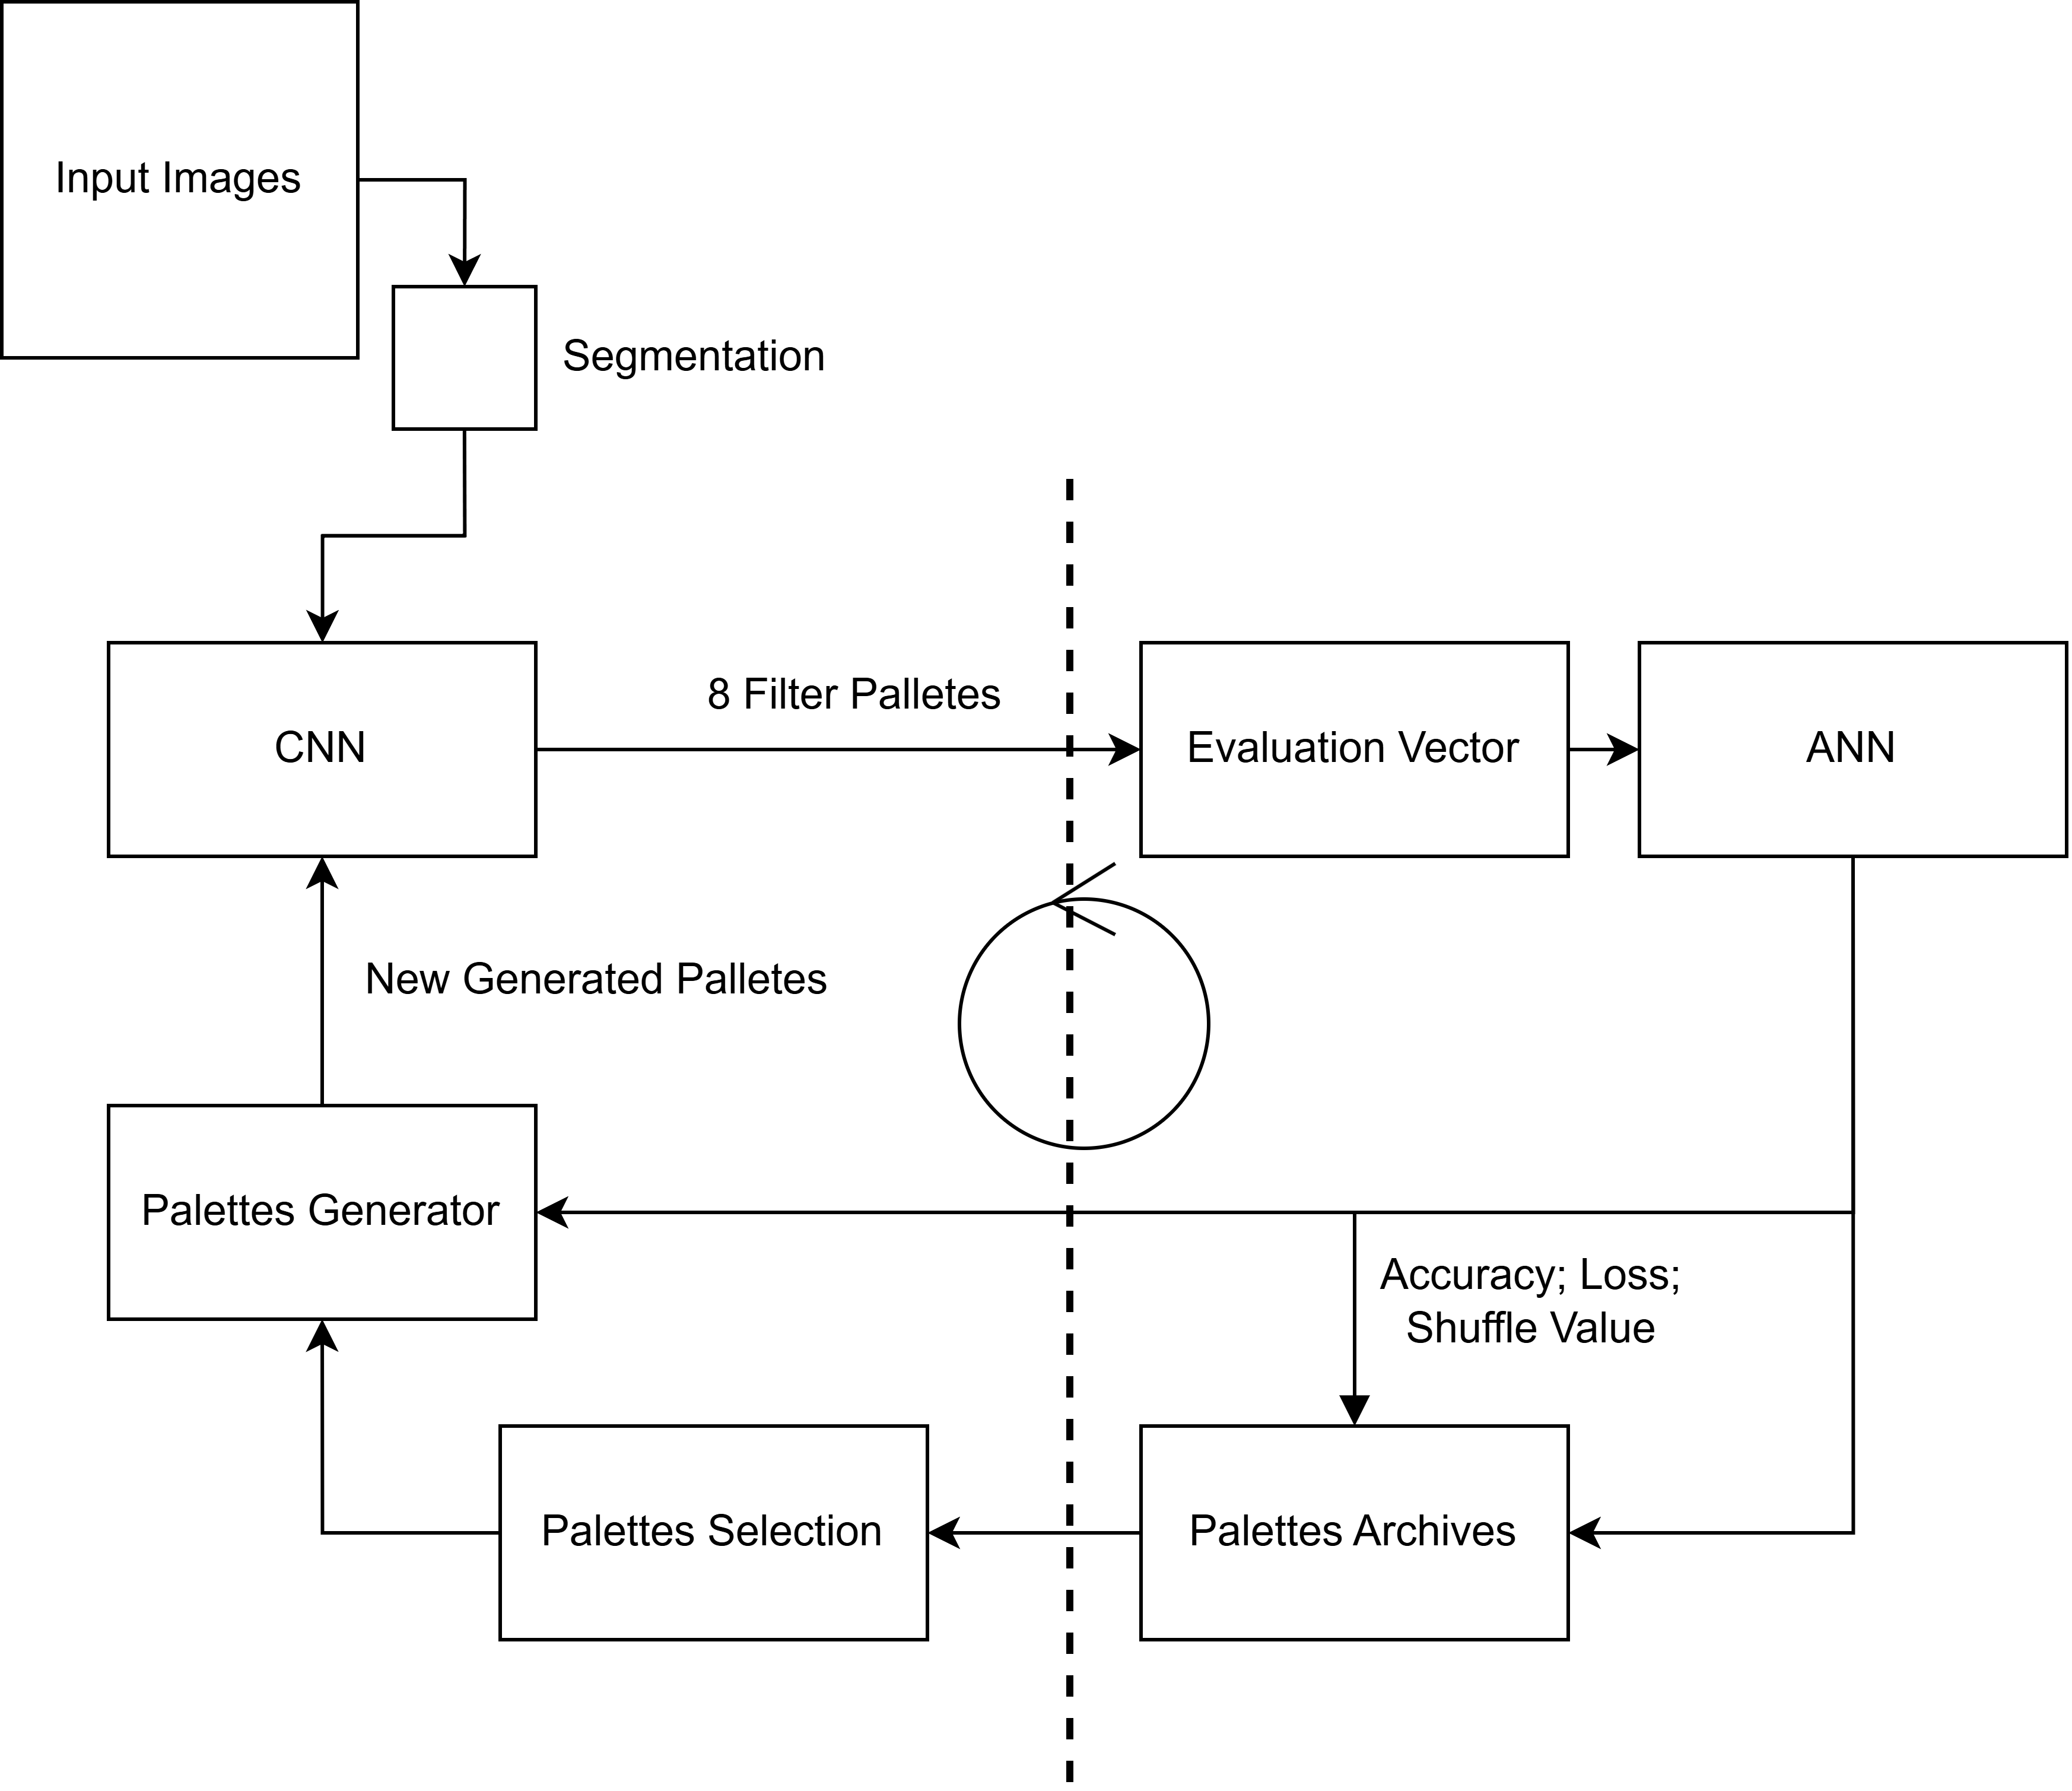
\includegraphics[width=0.7\textwidth]{images/CLM1.png}
	\caption{Visualisasi mekanisme \textit{Correlation Learning Mechanism} (CLM) \cite{wozniak2021deep}}
	\label{gambar:clm1}
\end{figure}

Gambar kedua menampilkan secara lebih rinci bagian arsitektur CNN yang digunakan dalam sistem CLM. Diagram ini menunjukkan bagaimana citra input diproses melalui dua tahap pooling dan konvolusi secara berurutan, yaitu \textit{pooling} $4\times4$ yang menghasilkan 4 \textit{feature maps} melalui konvolusi, dilanjutkan dengan fungsi aktivasi ReLU, kemudian \textit{pooling} $3\times3$ yang menghasilkan 16 \textit{feature maps} melalui konvolusi berikutnya. Hasil akhir dari proses ini berupa \textit{feature maps} yang diringkas menjadi enam nilai statistik sebelum diteruskan ke \textit{Evaluation Vector} dan ANN untuk proses evaluasi lebih lanjut.

\begin{figure}[h]
	\centering
	\captionsetup{justification=centering}
	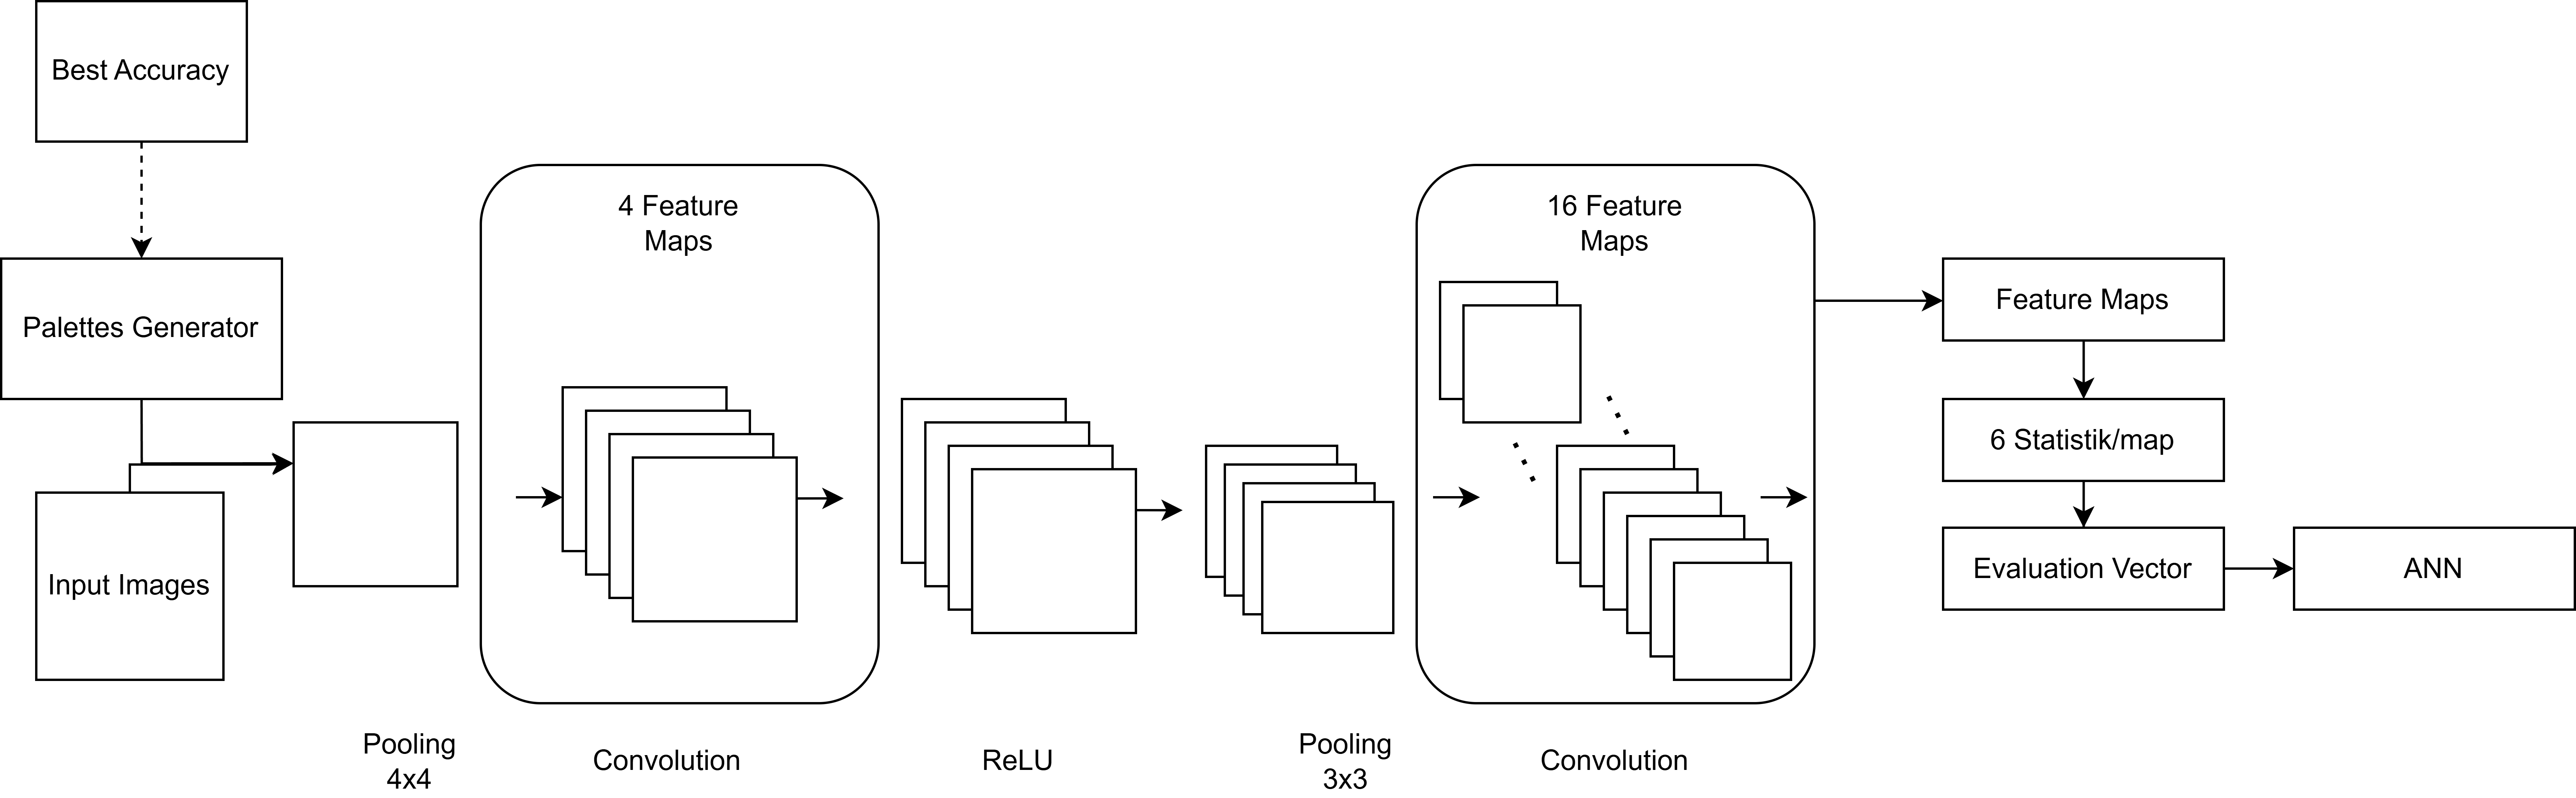
\includegraphics[width=0.7\textwidth]{images/CLM2.png}
	\caption{Visualisasi mekanisme \textit{Correlation Learning Mechanism} (CLM) \cite{wozniak2021deep}}
	\label{gambar:clm2}
\end{figure}

Alur kerja sistem secara menyeluruh dijelaskan sebagai berikut.

\begin{enumerate}
	\item Input CT Image\\
	Citra CT otak dimasukkan sebagai input awal ke dalam sistem.
	
	\item Segmentasi (64 fragmen)\\
	Citra input dibagi menjadi 64 fragmen berbentuk persegi agar dapat diproses secara paralel pada arsitektur multi-core/multi-thread.
	
	\item CNN (Pooling $4\times4$ $\rightarrow$ Konvolusi 4 fitur $\rightarrow$ ReLU $\rightarrow$ Pooling $3\times3$ $\rightarrow$ Konvolusi 16 fitur)\\
	Setiap fragmen citra diproses oleh CNN melalui dua blok konvolusi. Blok pertama terdiri dari operasi \textit{pooling} $4\times4$ dilanjutkan konvolusi yang menghasilkan 4 \textit{feature maps}, kemudian dilewatkan fungsi aktivasi ReLU untuk meratakan nilai piksel. Blok kedua terdiri dari \textit{pooling} $3\times3$ dilanjutkan konvolusi yang menghasilkan 16 \textit{feature maps}. Konfigurasi filter yang digunakan pada tiap lapisan konvolusi disebut \textit{palette}.
	
	\item Evaluation Vector (6 statistik: min, max, sum, median, mean, std)\\
	\textit{Feature maps} hasil keluaran CNN diringkas menjadi enam nilai statistik, yaitu nilai minimum, maksimum, jumlah, median, rata-rata aritmetika, dan standar deviasi, yang membentuk deskripsi numerik dari citra input.
	
	\item ANN ($[90]\text{-}[45]\text{-}[10]\text{-}[5]\text{-}[4]\text{-}[2]$, sigmoid, backpropagation/Adam)\\
	Vektor evaluasi dari CNN diteruskan ke ANN yang terdiri dari lima hidden layer dengan jumlah neuron $90, 45, 10, 5, 4$, dan $2$ pada layer keluaran. ANN menggunakan fungsi aktivasi sigmoid unipolar dan dilatih menggunakan algoritma \textit{backpropagation} maupun optimasi Adam untuk memperbarui bobot jaringan.
	
	\item Output: keputusan tumor terdeteksi atau tidak\\
	ANN menghasilkan keputusan akhir berupa klasifikasi biner, yaitu apakah tumor terdeteksi pada citra CT otak atau tidak.
	
	\item (loss, accuracy, shuffle value) disimpan ke Palettes Archives\\
	Nilai \textit{loss}, akurasi, dan \textit{shuffle value} yang dihasilkan dari proses evaluasi ANN disimpan ke dalam basis data arsip palette.
	
	\item Palettes Selection memilih palette terbaik\\
	Berdasarkan nilai \textit{loss} dan akurasi yang tersimpan, sistem memilih konfigurasi palette CNN dengan performa terbaik.
	
	\item Palettes Generator membangkitkan palette baru\\
	Palette terbaik yang telah dipilih digunakan sebagai dasar untuk menghasilkan konfigurasi palette baru bagi CNN.
	
	\item Dikirim kembali ke CNN untuk iterasi berikutnya\\
	Palette baru dikirimkan kembali ke CNN sebagai bagian dari mekanisme umpan balik, sehingga CNN dapat terus disesuaikan untuk mencapai hasil deteksi yang lebih optimal pada iterasi-iterasi selanjutnya.
\end{enumerate}

\subsection{Explainable CNN}
Model yang digunakan adalah CNN yang disederhanakan menggunakan Grad-CAM sebagai dasar \textit{pruning} layer, bukan sekadar alat visualisasi pasif.

\begin{figure}[h]
	\centering
	\captionsetup{justification=centering}
	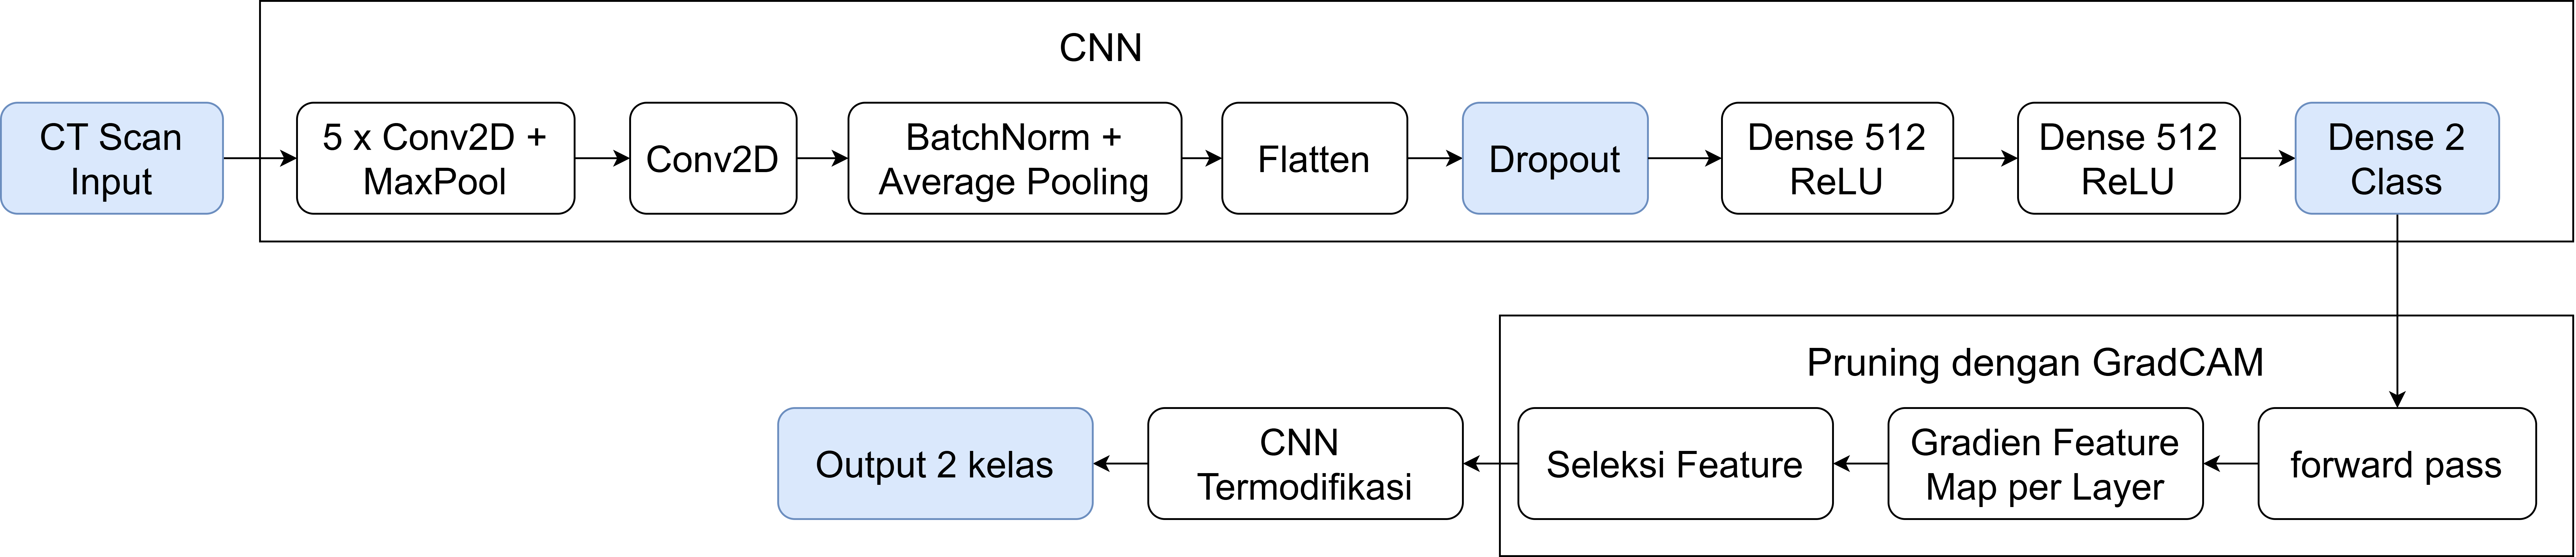
\includegraphics[width=0.85\textwidth]{images/before exp cnn.png}
	\caption{Arsitektur Model CNN + ANN}
	\label{gambar:beforeexpcnn}
\end{figure}

\begin{enumerate}
	\item Arsitektur CNN Termodifikasi
	Detail susunan lapisan (layer) dari arsitektur CNN yang diajukan dalam eksperimen ini adalah sebagai berikut:
	\begin{itemize}
		\item Conv2D + MaxPooling ($\times5$): Filter 8, 16, 32, 64, 128; kernel $3\times3$, \textit{padding same}, aktivasi ReLU; MaxPooling faktor 2 tiap blok.
		\item Conv2D Transisi: $1\times$ Lapisan Conv2D tambahan sebelum masuk ke tahap \textit{pooling} akhir.
		\item BatchNorm + Average Pooling: Normalisasi aktivasi diikuti dengan \textit{down-sampling} lanjutan.
		\item Flatten: Mengubah \textit{feature map} multi-dimensi menjadi vektor 1D.
		\item Dropout (Tambahan): Lapisan regulasi untuk mencegah \textit{overfitting} (Wojciuk dkk., 2024).
		\item $2\times$ Dense 512 + ReLU: Dua lapisan \textit{fully connected} dengan masing-masing 512 neuron dan aktivasi ReLU.
		\item Dense 2 Class (Tujuan): Lapisan output biner (2 kelas) dengan fungsi aktivasi untuk klasifikasi target.
	\end{itemize}
	
	\item Pruning Berbasis Grad-CAM dan Validasi
	Proses reduksi ukuran model dilakukan secara terukur melalui tahapan berikut:
	\begin{enumerate}
		\item \textit{Forward Pass}: Memproses citra input untuk menghasilkan prediksi kelas.
		\item Gradien \textit{Feature Map} per Layer: Melakukan \textit{backward pass} untuk menghitung gradien skor kelas terhadap \textit{feature map} tiap layer konvolusi. Gradien dirata-ratakan menjadi bobot $\alpha$, dikalikan \textit{feature map}, dijumlahkan, dan dilewatkan ke fungsi ReLU untuk memperoleh nilai kepentingan fitur.
		\item Seleksi Fitur: Menghitung rata-rata kepentingan tiap layer. Layer di bawah ambang batas (\textit{threshold} berupa nilai mean terendah antar-layer) akan dihapus.
		\item CNN Termodifikasi \& Output 2 Kelas: Arsitektur hasil \textit{pruning} dilatih ulang (\textit{fine-tuning}) hingga memproduksi keluaran final berupa Output 2 kelas.
	\end{enumerate}
	
	\item Perubahan Komponen
	Berdasarkan diagram alur eksperimen, terdapat komponen-komponen yang disesuaikan pada tugas akhir ini disorot dengan warna biru, meliputi:
	\begin{itemize}
		\item CT Scan Input: Modifikasi fokus modalitas medis utama dari citra MRI menjadi CT Scan. Perubahan ini dilakukan untuk menyessuaikan tujuan utama penelitian untuk menciptakan model pendeteksian otak menggunakan citra medis CT Scan.
		\item Dropout Layer: Penambahan lapisan \textit{Dropout}  setelah proses \textit{Flattening}. Berdasarkan riset Wojciuk dkk. (2024),  \textit{dropout} efektif dalam mencegah masalah \textit{overfitting} pada model pembelajaran mendalam yang memiliki dataset medis dengan distribusi atau kuantitas sampel yang terbatas.
		\item Dense 2 Class: Menyesuaikan ujung struktur model dari keluaran multi-kelas menjadi klasifikasi biner. Modifikasi pada \textit{Dense layer} dan \textit{Output} klasifikasi biner ini merupakan bentuk penyesuaian terhadap spesifikasi dan tujuan dari penelitian ini.
	\end{itemize}
\end{enumerate}

\subsection{EfficientNetB0}

%\begin{figure}[h]
%	\centering
%	\captionsetup{justification=centering}
%	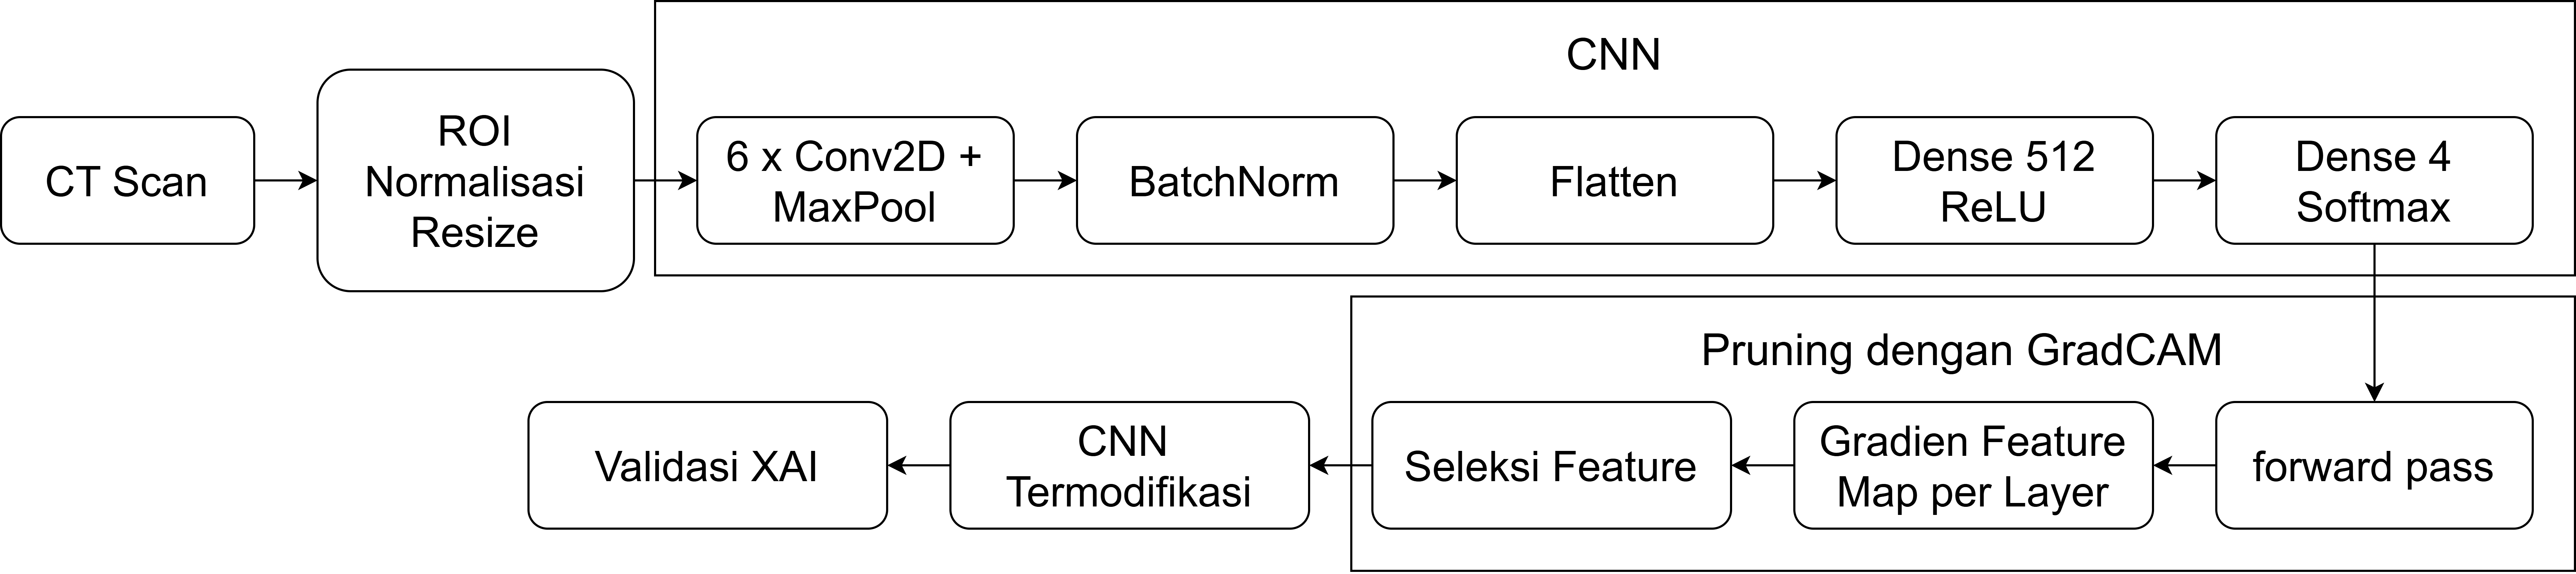
\includegraphics[width=0.7\textwidth]{images/before_exp_cnn.png}
%	\caption{Arsitektur Model CNN + ANN}
%	\label{gambar:beforetransferlearning}
%\end{figure}

\subsection{hyperparameter \textit{tuning}}
Pemilihan hyperparameter tidak memiliki standar universal yang menjamin hasil optimal untuk setiap tugas klasifikasi. Berdasarkan penelitian Wojciuk dkk. (2024), meskipun learning rate dan ukuran gambar input secara umum memberikan dampak terbesar pada performa model, tingkat signifikansi dari hyperparameter sangat bervariasi bergantung pada karakteristik dataset yang digunakan. hyperparameter \textit{tuning} yang dilakukan adalah sebagai berikut.
\begin{enumerate}
	\item \textit{Learning Rate} (0.0001, 0.001, 0.01):
	Pada penelitian Wojciuk dkk. (2024), \textit{learning rate} yang diuji memiliki nilai antara 0.0001 hingga 0.03. Artikel tersebut mencatat bahwa \textit{learning rate} dengan nilai yang lebih rendah umumnya berkorelasi dengan performa model yang lebih tinggi.
	
	\item \textit{Batch Size} (16, 40, 64):
	Berdasarkan penelitian Wojciuk dkk. (2024), \textit{batch size} yang dicoba memiliki nilai 16, 40, dan 64. Walaupun artikel menemukan bahwa \textit{batch size} memiliki dampak yang sangat minim pada akurasi, artikel tersebut juga menjelaskan bahwa signifikansi parameter terhadap model bergantung kepada dataset yang digunakan sehingga dapat dilakukan eksperimen terhadap parameter-parameter lain.
	
	\item \textit{Dropout Rate} (0.1, 0.2, 0.3):
	Di sinilah terdapat perbedaan yang patut dicatat. Artikel Wojciuk dkk. menguji rentang 0.01 hingga 0.4 dan menemukan bahwa performa terbaik biasanya berada di rentang 0.1 hingga 0.3. Namun, nilai yang Anda pilih (terutama 0.5) sebenarnya merupakan standar yang sangat umum digunakan untuk arsitektur klasifikasi citra medis. Untuk tugas dengan kompleksitas fitur yang tinggi seperti deteksi tumor otak pada CT-\textit{Scan}, \textit{dropout} yang lebih besar sering kali diperlukan agar model tidak \textit{overfitting} terhadap pola spesifik dari data latih. 
\end{enumerate}

\subsection{Explainable AI}

Pada tugas akhir ini, terdapat modifikasi arsitektur terutama dalam \textit{palettes generator}. \textit{Palettes generator} yang terdapat pada sistem saat ini diganti menggunakan XAI yang akan memberikan penjelasan yang lebih baik. Terdapat penambahan arsitektur yang akan dilakukan, yaitu \cite{Cea2017GradCAM}:

\begin{enumerate}
	\item GradCAM++ untuk Explainable CNN \\
	\begin{enumerate}
		\item Ekstraksi Fitur dan Logit (Model Hooking): Kode membuat model ekstraksi ganda (grad\_model) yang secara simultan menangkap matriks fitur dari lapisan konvolusi terakhir (conv6 berdimensi 7x7x256) dan skor kelas prediksi dalam bentuk raw logit (lapisan Dense dengan activation='linear').
		\item Aliran Gradien Mundur (Backward Pass): Dengan menggunakan konteks tf.GradientTape, kode memantau matriks konvolusi (conv\_out) dan menghitung turunan parsial pertama (grads) dari skor kelas spesifik terhadap matriks tersebut.
		\item Kalkulasi Bobot Grad-CAM++ (Closed-form): Kode tidak benar-benar menghitung turunan kedua dan ketiga melalui diferensiasi otomatis TensorFlow, melainkan mengkuadratkan (grads\_sq = grads$^2$) dan memangkatkan tiga turunan pertamanya (grads\_cube = grads$^3$). Perhitungan ini dikombinasikan dengan total aktivasi fitur (A\_sum) untuk mendapatkan koefisien bobot tiap piksel secara spasial (alpha).
		\item Seleksi Gradien Positif: Koefisien alpha dikalikan secara eksklusif dengan gradien yang bernilai positif saja melalui aktivasi ReLU lalu dijumlahkan untuk mendapatkan bobot (weights) akhir tiap peta fitur (feature map).
		\item Formasi Heatmap: Matriks conv6 dikalikan dengan pembobot liniernya, dijumlahkan di seluruh sumbu kedalaman (axis=-1), dan dilewatkan pada fungsi ReLU untuk membuang nilai aktivasi negatif. Hasilnya adalah matriks saliency mentah berukuran 7x7.
		\item Normalisasi \& Overlay: Matriks 7x7 tersebut dinormalisasi ke rentang nilai [0, 1] secara presisi (dengan parameter epsilon EPS untuk menghindari pembagian dengan nol). Matriks ini lalu diperbesar (upsampling) menjadi resolusi citra masukan (224x224) menggunakan interpolasi gambar standar (cv2.resize), diwarnai dengan palet termal (JET), dan ditimpa di atas citra RGB asli (cv2.addWeighted).
	\end{enumerate}
	
	\item GradCAM untuk Transfer Learning EfficientB0 \\
	Alur kerjanya terdiri dari lima langkah GradCAM untuk Transfer Learning adalah berikut:
	\begin{enumerate}
		\item Forward Pass: Gambar MRI diproses melalui jaringan (\textit{forward pass}) hingga mencapai lapisan konvolusi yang ditargetkan untuk menghasilkan \textit{feature maps} (peta fitur).
		\item Komputasi Gradien: Jaringan kemudian menghitung gradien dari kelas target keluaran (misalnya probabilitas untuk kelas Glioma) terhadap \textit{feature maps} yang dihasilkan pada tahap sebelumnya.
		\item Pooling (Penggabungan): Nilai gradien tersebut dirangkum (\textit{pooled}) melintasi dimensi lebar dan tinggi untuk menghasilkan sekumpulan bobot pada setiap \textit{feature map}. Bobot ini secara matematis menunjukkan tingkat kepentingan setiap peta fitur terhadap kelas prediksi.
		\item Generasi Heatmap: Model melakukan kombinasi berbobot (\textit{weighted combination}) dari \textit{feature maps} pada \textit{forward pass} menggunakan bobot yang telah dihitung. Langkah ini menghasilkan \textit{heatmap} (peta panas) mentah.
		\item Superimposisi Visual: Heatmap tersebut dihamparkan di atas gambar MRI asli untuk memberikan representasi visual yang secara eksplisit menyoroti wilayah anatomis yang paling memengaruhi model dalam menebak jenis tumor.
	\end{enumerate}
\end{enumerate}

\section{Rancangan Evaluasi}
\subsection{Evaluasi Model}
Untuk menilai kinerja klasifikasi model, penelitian ini menggunakan evaluasi yang sama dengan evaluasi model yang dilakukan oleh penelitian x dan penelitian y, yaitu:

\begin{enumerate}
	\item Akurasi (\textit{Accuracy}):
	Mengukur rasio prediksi benar secara keseluruhan dengan membandingkan prediksi positif dan negatif yang benar (\textit{True Positives} dan \textit{True Negatives}) terhadap total seluruh data.
	\item Presisi (\textit{Precision}):
	Mengukur ketepatan prediksi positif yang dihasilkan oleh model.
	\item \textit{Recall}:
	Mengukur kemampuan model dalam menemukan semua sampel positif yang sebenarnya.
	\item Spesifisitas (\textit{Specificity}):
	Mengukur kemampuan model dalam mengidentifikasi hasil negatif dengan benar (tercantum dalam hasil evaluasi di Tabel 5 dan visualisasi metrik).
	\item \textit{F1-Score}:
	Mengukur keseimbangan model menggunakan rata-rata harmonik dari Presisi dan \textit{Recall}.
\end{enumerate}

\subsection{Evaluasi XAI}
Evaluasi terhadap \textit{Explainable Artificial Intelligence} (XAI) bertujuan untuk memastikan bahwa model tidak hanya akurat, tetapi juga transparan, dapat diinterpretasikan, dan dapat dipercaya untuk adopsi di dunia nyata. Evaluasi kualitas dari penjelasan XAI ini akan dilakukan sebagai berikut:

\begin{enumerate}
	\item \textit{Ground Truth Comparison}\\
	Penelitian ini menerapkan metrik XAlign yang diusulkan oleh \textcite{muhammad2025heatmap} dengan penjelasan yang dapat dilihat pada Bab \ref{chap:studi-literatur}. Skor XAlign akan dihitung untuk setiap hasil prediksi Grad-CAM menggunakan persamaan:
	\begin{equation}
		XAlign = \alpha \cdot WRO + \beta \cdot BAS - \gamma \cdot DP
	\end{equation}
	Nilai bobot akan diatur mengikuti konfigurasi standar berdasarkan penelitian tersebut, yaitu $\alpha=0,5$, $\beta=0,4$, dan $\gamma=0,1$. Skor XAlign yang mendekati 1,0 akan mengindikasikan bahwa Grad-CAM berhasil menghasilkan penjelasan yang sangat selaras dengan diagnosis klinis.
	
	Sebagai kriteria keberhasilan, penelitian ini mengacu pada performa Grad-CAM yang dilaporkan dalam studi literatur pada \textit{dataset} neuro-onkologi (TCGA-LGG). Metode yang digunakan mencatat skor rata-rata XAlign sebesar $64,1\%$ \autocite{muhammad2025heatmap}. Oleh karena itu, tugas akhir ini menargetkan capaian skor XAlign $\geq 0,641$ sebagai batas minimal validitas penjelasan yang dihasilkan model.
	
	\item Evaluasi Kualitatif\\
	Sebagai pelengkap data kuantitatif XAlign, dilakukan evaluasi kualitatif perbandingan visual \textit{side-by-side} tetap akan dilakukan antara citra asli, \textit{ground truth mask}, dan \textit{heatmap} Grad-CAM untuk analisis kasus per kasus. Setelah dilakukan analisis visual dari heatmap, dilakukan analisis penyebab gradcam masih belum sesuai dengan \textit{ground truth mask}, seperti dari kualitas gambar, posisi tumor, dan ukuran tumor.
\end{enumerate}